\section{Implementation} \label{sec:implementation}
This section presents the implementation of our robotics architecture design. Our program, called the {\it Scene Generator}, has been created to assist in the creation of Turtle format files for expressing data in the Resource Description Framework (RDF) data model~\cite{beckett2014rdf} that provides scene information for SkiROS. Scenes describe the entities in the robot's environment that it is able to reason about. These entities take the form of named individuals (i.e. concrete instances) of the classes defined in the {\tt paintbot} ontology. The Scene Generator provides a convenient interface for specifying the named individuals for any given environment. The program generates a file in the Turtle format that is ready to be loaded by SkiROS. Figure \ref{fig:scene_generator} demonstrates a sample of the graphical component of the scene generator.

\begin{figure}
    \centering
    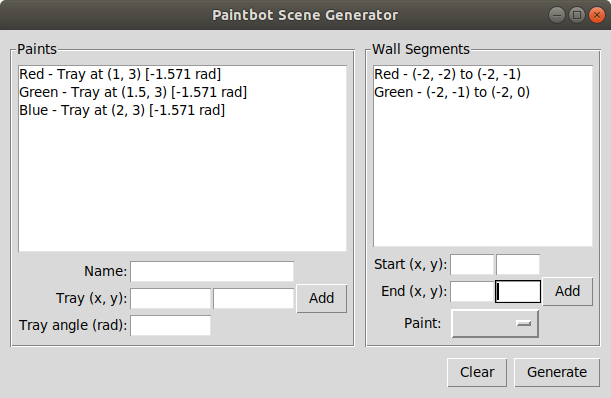
\includegraphics[width=0.7\linewidth]{images/scene_generator.png}
    \caption{The Scene Generator application designed for this project. The left panel allows paints and trays to be specified while the right panel allows wall segments to be specified. This example shows the configuration for one of the scenes used to test the platform.}
    \label{fig:scene_generator}
\end{figure}

The scene generator currently supports the specification of paints and walls. When specifying a paint, the user provides its name and the location and orientation of the tray that contains it. When specifying a wall, the user provides the two endpoints of the wall, $w_0$ and $w_1$, and the color it is to be painted. The line segment defined by the two endpoints is divided into \SI{9}{inch} sections (note that \SI{9}{inches} is a very common size for paint rollers) and the center points of the sections are adjusted so that no section extends past either end of the line segment. This may result in some overlap between sections. The face of the wall that needs to be painted is perpendicular to the line segment and is defined by the following equation:
\[w_\theta = \atantwo(w_{1y} - w_{0y}, w_{1x} - w_{0x}) - \frac{\pi}{2}\]
Any number of paints and walls may be specified using the Scene Generator.

The graphical interface provided by SkiROS is the primary means of interacting with the robot at runtime for this project. More specifically, there are two skills used to perform goal planning and execution: {\tt task\_plan} and {\tt paintallwallsections}. {\tt task\_plan} is provided by SkiROS and allows a goal state in PDDL to be specified. This skill sends the goal state to the TFD planner and executes the generated plan. An example goal utilizing the {\tt paintbot} ontology, and the one used in all the simulations, is {\tt (forall (?w - paintbot:WallSection) (Painted ?w))}. This goal declares that every wall section in the scene must ultimately have the {\tt Painted} property, which is assigned to a wall section upon successful completion of the ApplyPaint skill (see section \ref{sec:task_planning}).

The {\tt paintallwallsections} skill was created in response to observations made during development and testing. This skill causes the robot to paint every wall section in the scene by generating PDDL goals for batches of $10$ sections and invoking the {\tt task\_plan} skill for each batch. {\tt paintallwallsections} was created to serve two primary purposes: 1) to reduce planning times (see section \ref{sec:results_plan}) and 2) as an exploratory exercise in dynamic planning.

\begin{figure}
    \centering
    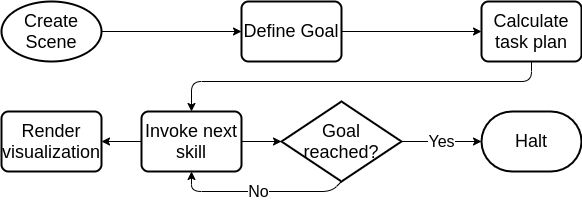
\includegraphics[width=1.0 \linewidth]{images/process_2.png}
    \caption{The general process of using the platform, from generating a scene through the robot executing the tasks to achieve the specified goal.}
    \label{fig:process}
\end{figure}

Figure \ref{fig:process} depicts a high-level overview of the process involved in operating the robot. First, a scene file in Turtle format needs to be generated that represents the entities in the construction environment. Currently, this needs to be manually done for each new environment the robot will operate in, though work can be done to automate this step. Second, a goal state needs to be provided, as described above. Third, the planner uses the scene information and goal state to calculate the task plan. Finally, the robot executes all skills in the task plan in order.

Figure \ref{fig:implement} illustrated the implementation of our robotic architecture. %Note that the orientation of the room is roughly the same within both images.
Figure \ref{fig:implement} (a) shows the simulation environment, and (b) shows the robot loading paint during the execution of the LoadPaint skill. Then, we demonstrate the various components of the Navigation Stack at runtime in Figure~\ref{fig:implement} (c). Figure~\ref{fig:implement} (d) visualized the  line of sight of the laser. In this scenario, the robot has loaded the roller with paint and is attempting to navigate to a wall it has not observed before on the left side of the image. The room can be seen to be partially mapped by the GMapping algorithm. The light grey regions have been observed with the laser and marked as clear, the black regions have been observed and marked as obstacles, and the dark grey areas have not been observed by the robot. The robot's pose in this visualization is where the AMCL algorithm has localized the robot within the map. The green and red lines are the global and local trajectories, respectively, planned out by the TEB algorithm.


\begin{figure}
    \centering
    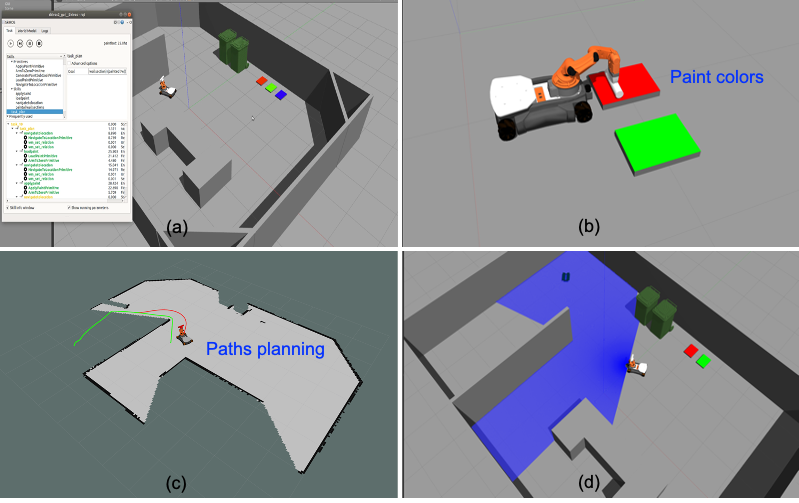
\includegraphics[width=1.0 \linewidth]{images/implement.png}
    \caption{The implementation of our robotic architecture. (a) Simulated room containing three paint trays along the ``northern'' wall, walls with varying orientations, and a few obstacles. (b) The robot loading red paint from a tray. (c) Visualization of the robot's map of the room and path planning. The green and red lines are the global and local TEB trajectories, respectively. (d) Visualization of the line of sight of the laser, in blue.}
    \label{fig:implement}
\end{figure}
